\ifx \allfiles \undefined
\documentclass[12pt,a4paper,oneside]{article}

%% === CJK 套件 ===
\usepackage{CJKutf8,CJKnumb}                 % 中文套件
%% === AMS 標準套件 ===
\usepackage{amsmath,amsfonts,amssymb,amsthm} % 數學符號
%% === ===
\usepackage{algorithm}
\usepackage{listings}                        % 程式碼
%% === TikZ 套件 ===
\usepackage{tikz,tkz-graph,tkz-berge}        % 繪圖
\usepackage{multicol}
%% == ==
\usepackage[unicode]{hyperref}
\usepackage{xcolor}
\hypersetup{
    colorlinks,
    linkcolor={blue!100!black},
    citecolor={blue!75!black},
    urlcolor={blue!50!black}
}
%% == 調整設定 ==
\usepackage{enumitem}                           % 修改 enumerate, item
\usepackage{bbding}
\usepackage{titletoc,titlesec,imakeidx}
%% == ==
\usepackage{newfloat}
\usepackage{caption,subcaption}
\usepackage{xkeyval,xargs}
\usepackage{ulem}
\usepackage{import}

%% === 設定 C++ 格式 ===
\lstset{%
  language=C++,             % 設定語言
  %% === 空白, tab 相關 ===
  tabsize=2,                % 設定 tab = 多少空白
  %showspaces=true,          % 設定是否標示空白
  %showtabs=true,            % 設定是否標示 tab
  %tab=\rightarrowfill,      % 設定 tab 樣式
  %% === 行數相關 ===
  numbers=left,             % 行數標示位置
  stepnumber=1,             % 每隔幾行標示行數
  numberstyle=\tiny,
  %breaklines=true,          % 設定斷行
  %% === 顏色設定 ===
  basicstyle=\ttfamily,
  keywordstyle=\color{blue}\ttfamily,
  stringstyle=\color{red!50!brown}\ttfamily,
  commentstyle=\color{green!50!black}\ttfamily,
  %identifierstyle=\color{black}\ttfamily,
  emphstyle=\color{purple}\ttfamily,
  extendedchars=false,
  texcl=true,
  moredelim=[l][\color{magenta}]{\#},
  captionpos=b,
  %% === 其他 ===
  %frame=single
}

% ===============================================
%
%  設定頁面格式
%
% ===============================================
%% === 設定頁面格式 ===
%\hoffset         = 10pt                      % 水平位移,預設為 0pt
\voffset         = -15pt                     % 垂直位移,預設為 0pt
\oddsidemargin   = 0pt                       % 預設為 31pt
%\topmargin       = 20pt                      % 預設為 20pt
%\headheight      = 12pt                      % header 的高度,預設為 12pt
%\headsep         = 25pt                      % header 和 body 的距離,預設為 25pt
\textheight      = 620pt                     % body 內文部分的高度,預設為 592pt
\textwidth       = 450pt                     % body 內文部分的寬度,預設為 390pt
%\marginparsep    = 10pt                      % margin note 和 body 的距離,預設為 10pt
%\marginparwidth  = 35pt                      % margin note 的寬度,預設為 35pt
%\footskip        = 30pt                      % footer 高度 + footer 和 body 的距離,預設為 30pt

%% ==  ==
\DeclareFloatingEnvironment[fileext=frm,placement={!ht},name=Frame]{code}
\captionsetup[code]{labelfont=bf}

\makeindex

\linespread{1.14}

\begin{document}
\begin{CJK}{UTF8}{bkai}

\subimport{./config/}{docsetting.tex}
\setcounter{section}{1}

\fi

\tikzset{bit block/.style={
	draw,
	rectangle,
	minimum height=\myht*\sz,
	minimum width=\mywd*\sz
}}
\tikzset{line arrow/.style={
	thick,
	latex-latex,
	-triangle 45
}}

\section{程式架構解析}

\paragraph{}這一節主要延續上一節的思維,但著重在了解程式如何執行,利用這些知識順利寫出\textbf{架構簡潔}、\textbf{容易除錯}程式。因此在這一節練習題較少,大多是\textbf{重要的觀念}。

\paragraph{本節目標}

\subsection{位址與指標}

\subsubsection{溢位現象}

\paragraph{}以下程式碼會發生什麼現象?
\begin{code}[h!]
\centering
\begin{tabular}{c}
\begin{lstlisting}
int x = 2147483647;
cout << x + 1 << endl;
\end{lstlisting}
\end{tabular}
\caption{產生溢位的程式碼}
\label{program:struct:code:overflow}
\end{code}

\paragraph{}上一節提到 \lstinline!int! 的定義為「至少 2 個位元組」,若讀者的 \lstinline!int! 也是 4 個位元組的話,那麼就會得到 \lstinline!-2147483648!!這種現象我們稱為\index{溢位}{\textbf{溢位現象 (Overflow)}}。我們從二進位下看這段程式,會比較了解:

\begin{table}[h!]
\centering
\begin{tabular}{|c|c|c|c|}
\hline
$01111111$ & $11111111$ & $11111111$ & $11111111$\\
\hline
\end{tabular}
\caption{\lstinline!2147483647!}
\label{program:struct:table:binary:2147483647}
\end{table}

\paragraph{}表 \ref{program:struct:table:binary:2147483647} 表示 \lstinline!2147483647! 在 \texttt{C++} 當中如何儲存,讀者可以驗證 $2147483647=2^{31}-1$。若我們此時對 \lstinline!2147483647! 加 \lstinline!1!,就會得到下面的結果:

\begin{table}[h!]
\centering
\begin{tabular}{|c|c|c|c|}
\hline
${\color{red}1}0000000$ & $00000000$ & $00000000$ & $00000000$\\
\hline
\end{tabular}
\caption{\lstinline!2147483647 + 1!}
\end{table}

\paragraph{}用 \lstinline!int! 的儲存方法驗證,這個數字就是 \lstinline!-2147483648!,也就是 $-2^{32}$!為什麼會這樣子呢?
\paragraph{}大體上,表示資料的記憶體大小是\textbf{有限}的,那麼就會有以下兩種事情發生:
\begin{itemize}
\item 只能表示\textbf{有限多種}資料。例如:\lstinline!int! 通常是 4 個位元組,也就是 $4\times{8}=32$ 個位元,每個位元只能表示 \lstinline!0! 和 \lstinline!1! 兩種可能性,則最多只能表示 $2^{32}$ 種整數。這些可能性切一半,$2^{31}$ 個表示負整數,$2^{31}$ 表示非負整數,其中有一個 $0$,剩下 $2^{31}-1$ 個是正整數,因此 \lstinline!int! 的範圍就是介於 $-2^{31}$ 到 $2^{31}-1$。
\item \textbf{精確度}的限制。資料型態 \lstinline!double! 是以 \href{https://zh.wikipedia.org/wiki/IEEE_754}{IEEE 754} 為標準,有 8 個位元組,最多只能表示 $2^64$ 種小數。因為在標準中,以 53 個位元儲存尾數,故有 52 位有效數字,精確度為 $\log{2^{52}}\approx{15.95}$ 位十進位有效數字 (\lstinline!float! 則為 7 位)。
\end{itemize}

\begin{table}[h!]
\centering
\begin{tabular}{|c|c|c|c|}
\hline
\textbf{資料型態} & \textbf{位元組} & \textbf{通常下界} & \textbf{通常上界}\\
\hline\hline
\lstinline!char!      & 1 & $-128$        & $127$       \\
\hline
\lstinline!short!     & 2 & $-32768$      & $32767$     \\
\hline
\lstinline!int!       & 4 & $-2147483648$ & $2147483647$\\
\hline
\lstinline!long long! & 8 & $-9223372036854775808$ & $9223372036854775807$\\
\hline
\lstinline!float!     & 4 & $-3.40282\times{10^{38}}$ & $3.40282\times{10^{38}}$\\
\hline
\lstinline!double!    & 8 & $-1.79769\times{10^{308}}$ & $1.79769\times{10^{308}}$\\
\hline
\lstinline!unsigned char!      & 1 & $0$ & $255$\\
\hline
\lstinline!unsigned short!     & 2 & $0$ & $65535$\\
\hline
\lstinline!unsigned int!       & 4 & $0$ & $4294967295$\\
\hline
\lstinline!unsigned long long! & 8 & $0$ & $18446744073709551615$\\
\hline
\end{tabular}
\caption{資料型態上下界}
\label{program:struct:table:datatype:limit}
\end{table}

\paragraph{}表 \ref{program:struct:table:datatype:limit} 表示每一種資料型態常見的上下界範圍,其中 \lstinline!unsigned! 類型代表「\textbf{不帶負號}」,也就是說 \lstinline!unsigned! 系列會把所有符號拿去表示非負數。
\paragraph{}此外,需要注意的有幾點:
\begin{itemize}
\item \lstinline!int! 的上限是 \lstinline!2147483647!,用十六進位表示為 \lstinline!0x7FFFFFFF!
\item \lstinline!long long! 範圍大概是 $-9\times{10^{18}}$ 到 $9\times{10^{18}}$ 之間
\item \lstinline!double! 的範圍介於 $-{10}^{308}$ 至 ${10}^{308}$ 左右
\end{itemize}
\paragraph{}這些範圍可以在標頭檔 \index{標頭檔!climits}{\lstinline!<climits>!} 和 \index{標頭檔!cfloat}{\lstinline!<cfloat>!} 當中查詢到,實際範圍會依據不同計算機而有差異,查詢的方法自行 google,這裡不贅述。

\subsubsection{記憶體}

\paragraph{}上一節提到\index{位元}{位元}和\index{位元組}{位元組}以及 \lstinline!sizeof! 等觀念,接下來要進入有關\index{記憶體}{\textbf{記憶體}}的部分。首先,我們常常提到的記憶體有分廣義和狹義,廣義的記憶體可以指稱所有儲存資料的設備,表 \ref{program:struct:table:hierarchical:memory} 列出計算機中常用的儲存設備:

\begin{table}[h!]
\centering
\begin{tabular}{|c|c|c|c|c|}
\hline
\textbf{種類}                                          & \textbf{原文} & \textbf{存取速度} & \textbf{容量} & \textbf{用途}                                              \\
\hline\hline
\color{blue}\textbf{暫存器} & Register & 1 CPU  週期 & 數百 Bytes 內 & \begin{tabular}[c]{@{}c@{}}CPU 內部暫存\\ 運算的資料\end{tabular}   \\
\hline
快取記憶體 & Cache & 數十 CPU 週期 & 數十 MB 內 & \begin{tabular}[c]{@{}c@{}}協調 CPU 和\\ 主記憶體的速度\end{tabular} \\
\hline
\color{red}\textbf{主記憶體} & Main Memory & 數百 CPU 週期 & 8 GB 左右 & \begin{tabular}[c]{@{}c@{}}執行程式、\\ 暫存資料等\end{tabular}      \\
\hline
\color{blue}\textbf{\begin{tabular}[c]{@{}c@{}}碟盤設備\\ (硬碟、光碟)\end{tabular}} & Disk Storage & 數百萬 CPU 周期 & 數 TB          & \begin{tabular}[c]{@{}c@{}}永久儲存\\ 程式、資料\end{tabular}       \\
\hline
\end{tabular}
\caption{廣義的記憶體,又稱為\textbf{記憶體階層} (2016 年資料)}
\label{program:struct:table:hierarchical:memory}
\end{table}

\paragraph{}狹義的記憶體就是\textbf{主記憶體},俗稱「\index{記憶體}{\textbf{記憶體}}」,程式在開始運行前,會將存在硬碟當中的程式資料移到記憶體當中,才會執行程式。

\subsubsection{位址}

\paragraph{}主記憶體可以看做是一條很長、連續的位元組,程式執行時,會佔據其中一個區塊,如圖 \ref{program:struct:fig:memory:and:program}:

\begin{figure}[h!]
\centering
\begin{tikzpicture}
\edef\mywd{2}
\draw (0,0) rectangle (13,\mywd);
\filldraw[black!40!white,draw=black] (0,0) rectangle (3,\mywd) node[black,pos=0.5] {作業系統};
\filldraw[black!30!white,draw=black] (3,0) rectangle (4,\mywd) node[black,pos=0.5] {程式};
\filldraw[black!30!white,draw=black] (5,0) rectangle (7,\mywd) node[black,pos=0.5] {程式};
\filldraw[black!30!white,draw=black] (7,0) rectangle (9,\mywd) node[black,pos=0.5] {程式};
\node at (-1,.5*\mywd) {記憶體};
\end{tikzpicture}
\caption{記憶體與程式}
\label{program:struct:fig:memory:and:program}
\end{figure}

\paragraph{}記憶體可以比作「\textbf{土地}」,一開始有一大片未經使用的土地,由作業系統和程式去分配用途 (當成 \lstinline!int!、\lstinline!double! 等)。為了方便管理記憶體,計算機會幫每個{\color{blue}\textbf{位元組}}標記「\textbf{地址}」,在此我們就稱為「\index{位址}{\color{red}\textbf{位址}}」。
\paragraph{}位元組是擁有地址的{\color{blue}\textbf{最小單位}},單個位元並沒有位址。

\paragraph{取址運算子}位址是一個數字,同常以十六進位表示,如果要知道一個變數的位址,可以使用\index{取址運算子}{取址運算子} \lstinline!&!,例如程式碼 \ref{program:struct:code:address}:

\begin{code}[h!]
\centering
\begin{tabular}{c}
\begin{lstlisting}
int a = 16;
cout << "Address of a = " << &a << endl;
\end{lstlisting}
\end{tabular}
\caption{印出 \lstinline!a! 的位址}
\label{program:struct:code:address}
\end{code}

\paragraph{}筆者的執行結果為:\lstinline!Address of a = 003FF07C!,代表變數 \lstinline!a! 實際的位址是在 \lstinline!0x003FF07C! 的位元組,相當於是他的「\textbf{門牌號碼}」,因為 \lstinline!int! 通常為 4 個位元組,因此會佔據 \lstinline!0x003FF07C!、\lstinline!0x003FF07D!、\lstinline!0x003FF07E!、\lstinline!0x003FF07F! 這四個位元組。如圖 \ref{program:struct:fig:int:address}:

\begin{figure}[h!]
\centering
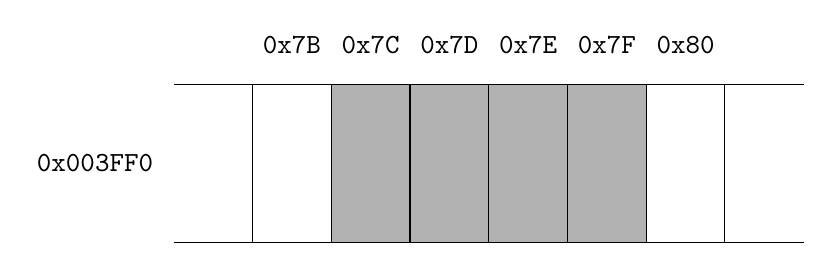
\begin{tikzpicture}
\def\arr{7B,7C,7D,7E,7F,80};
\draw (0,0) -- (8,0);
\draw (0,2) -- (8,2);
\edef\myleft{0}
\edef\myright{0}
\edef\mypos{0}
\foreach \item [count=\i] in \arr
{
	\ifthenelse{1<\i \AND \i<6}{%
		\fill[black!30!white] (\i,0) rectangle (\i+1,2);
	}{}
	\draw (\i,0) rectangle (\i+1,2);
	\node at (\i+0.5,2.5) {\texttt{0x\item}};
}
\node at (-1,1) {\texttt{0x003FF0}};
\end{tikzpicture}
\caption{變數 \lstinline!a! 實際的記憶體位置}
\label{program:struct:fig:int:address}
\end{figure}

\paragraph{}這個結果會因為不同機器、每次程式執行分配的記憶體而不同 (總之就是\textbf{不一定}啦!(╯°□°)╯︵ ╧╧),但概念是相同的。

\paragraph{大字節序和小字節序}但是我們要怎麼知道變數 \lstinline!a! 實際怎麼儲存在記憶體中呢?很多人會以為像是圖 \ref{program:struct:fig:big:endian:16}:

\begin{figure}[h!]
\centering
\begin{tikzpicture}
\def\sz{3mm}
\def\mywd{7.5}
\def\myht{2.3}
\def\addr{7C,7D,7E,7F};
\def\arr{$00000000$,$00000000$,$00000000$,$00001000$};
\foreach \item [count=\i] in \arr
{
	\node[bit block] at (\i*\mywd*\sz,0) {\item};
}
\foreach \item [count=\i] in \addr
{
	\node at (\i*\mywd*\sz,.65) {\texttt{0x\item}};
}
\node at (0,0) {\texttt{0x003FF0}};
\end{tikzpicture}
\caption{大字節序儲存方法}
\label{program:struct:fig:big:endian:16}
\end{figure}

\paragraph{}但這個說法不完全對,圖 \ref{program:struct:fig:big:endian:16} 的儲存方法被稱為「\textbf{大字節序} (Big Endian)」,也就是 \lstinline!int! 的高位數會儲存在位址\textbf{比較小}的地方。
\paragraph{}另一種跟他相對的稱為「\textbf{小字節序} (Little Endian)」,也就是數字的高位數儲存在位址比較大的地方。例如用整數 \texttt{0x12345678} 來表示這兩種儲存方法的差異如圖 \ref{program:struct:fig:big:endian} 和 \ref{program:struct:fig:little:endian}:

\begin{figure}[h!]
\centering
\begin{subfigure}{0.4\textwidth}
  \centering
  \begin{tikzpicture}
\def\sz{3mm}
\def\mywd{4.5}
\def\myht{2.3}
\def\addr{7C,7D,7E,7F};
\def\arr{12,34,56,78};
\foreach \item [count=\i] in \arr
{
	\node[bit block] at (\i*\mywd*\sz,0) {\texttt{0x\item}};
}
\foreach \item [count=\i] in \addr
{
	\node at (\i*\mywd*\sz,.65) {\texttt{0x\item}};
}
  \end{tikzpicture}
  \caption{以大字節序儲存}
  \label{program:struct:fig:big:endian}
\end{subfigure}
~
\begin{subfigure}{0.4\textwidth}
  \centering
  \begin{tikzpicture}
\def\sz{3mm}
\def\mywd{4.5}
\def\myht{2.3}
\def\addr{7C,7D,7E,7F};
\def\arr{78,56,34,12};
\foreach \item [count=\i] in \arr
{
	\node[bit block] at (\i*\mywd*\sz,0) {\texttt{0x\item}};
}
\foreach \item [count=\i] in \addr
{
	\node at (\i*\mywd*\sz,.65) {\texttt{0x\item}};
}
  \end{tikzpicture}
  \caption{以小字節序儲存}
  \label{program:struct:fig:little:endian}
\end{subfigure}
\caption{\texttt{0x12345678} 不同儲存方法}
\label{program:struct:fig:big:little:endian}
\end{figure}

\paragraph{}除此之外,還有一類是「混合字節序 (Middle Endian)」,是大字節序和小字節序混用或者是其他的狀況,這裡不贅述。
\paragraph{}無論是大字節序還是小字節序,在程式當中都是表示「\texttt{0x12345678}」這個數字,這些儲存方法只是表示計算機\textbf{實際儲存資料}的差異,程式配置一塊記憶體用來儲存 \texttt{0x12345678},實際怎麼儲存在很多狀況下其實並不重要,但偶爾要做一些操作時,就會牽扯到這個概念。

\subsubsection{指標}

\paragraph{}\textbf{指標}是一個概念,他代表一個{\color{blue}\textbf{箭頭}}指向一塊記憶體。如圖 \ref{program:struct:fig:pointer}。

\begin{figure}[h!]
\centering
\begin{tikzpicture}
\def\arr{7B,7C,7D,7E,7F,80};
\draw (0,0) -- (8,0);
\draw (0,2) -- (8,2);
\edef\myleft{0}
\edef\myright{0}
\edef\mypos{0}
\foreach \item [count=\i] in \arr
{
	\draw (\i,0) rectangle (\i+1,2);
	\node at (\i+0.5,2.5) {\texttt{0x\item}};
}
\node at (-1,1) {\texttt{0x003FF0}};
\draw[line arrow] (2.5,4) -- (2.5,3);
\end{tikzpicture}
\caption{指標概念}
\label{program:struct:fig:pointer}
\end{figure}

\paragraph{}\texttt{C++} 是利用{\color{red}\textbf{儲存記憶體位址}}的方式實做指標,如何實現一個指標我們慢慢細說。
\paragraph{宣告}首先,程式碼 \ref{program:struct:code:pointer:variable} 宣告一個\textbf{指標變數} \lstinline!ptr!。

\begin{code}[h!]
\centering
\begin{tabular}{c}
\begin{lstlisting}
int *ptr;
\end{lstlisting}
\end{tabular}
\caption{宣告指標變數 \lstinline!ptr!}
\label{program:struct:code:pointer:variable}
\end{code}

\paragraph{}在此,宣告指標\textbf{變數}的規則和之前宣告變數都是相同的原則:\textbf{變數名稱}和\textbf{用途},此時 \lstinline!ptr! 的資料型態為 \lstinline!int*!,代表這是一個指向 \lstinline!int! 的指標。因為資料型態是 \lstinline!int*!,所以也可用程式碼 \ref{program:struct:code:pointer:variable:another} 的方式來宣告。

\begin{code}[h!]
\centering
\begin{tabular}{c}
\begin{lstlisting}
int* ptr;
\end{lstlisting}
\end{tabular}
\caption{宣告指標變數 \lstinline!ptr!}
\label{program:struct:code:pointer:variable:another}
\end{code}

\paragraph{}讀者要注意的一點是,當宣告多個指標變數時,不能寫成 \lstinline!int* ptr, ptr2!,在這個情形下,\texttt{C++} 會把 \lstinline!ptr2! 宣告成 \lstinline!int!,正確宣告多指標變數要像程式碼 \ref{program:struct:code:pointer:variable:multiple}。

\begin{code}[h!]
\centering
\begin{tabular}{c}
\begin{lstlisting}
int *ptr, *ptr2;
\end{lstlisting}
\end{tabular}
\caption{宣告多個指標變數}
\label{program:struct:code:pointer:variable:multiple}
\end{code}

\paragraph{賦值}剛剛說過,\texttt{C++} 指標的運作是讓指標變數儲存\textbf{位址},如果以之前變數 \lstinline!a! 的例子來說,我們知道變數 \lstinline!a! 的位址是 \texttt{0x003FF07C},若我們要把 \lstinline!ptr! 指向變數 \lstinline!a! 所在的記憶體,我們可以用先前講過的\textbf{取址運算子},得到 \lstinline!a! 的位址,如程式碼 \ref{program:struct:code:pointer:assignment}。

\begin{code}[h!]
\centering
\begin{tabular}{c}
\begin{lstlisting}
int a = 16;
int *ptr = &a;
\end{lstlisting}
\end{tabular}
\caption{指標的賦值}
\label{program:struct:code:pointer:assignment}
\end{code}

\paragraph{}程式碼 \ref{program:struct:code:pointer:assignment} 的實際狀況如圖 \ref{program:struct:fig:pointer:assignment}。

\begin{figure}[h!]
\centering
\begin{tikzpicture}
\def\myht{3};
\def\mywd{1};
\def\cont{0x003FF07C,16};
\def\addr{0x003FF080,0x003FF07C};
\def\name{\lstinline!ptr!,\lstinline!a!};
\foreach \item [count=\i] in \cont {
	\draw (5*\i,0) rectangle (5*\i+\myht,\mywd)%
		node[black,pos=.5] {\texttt{\item}};
	\ifthenelse{1<\i}{
		\draw[line arrow] (5*\i-5+\myht,0.5) -- (5*\i,0.5);
	}{}
}
\foreach \item [count=\i] in \addr {
	\node at (\myht/2+5*\i,-0.4) {\texttt{\item}};
}
\foreach \item [count=\i] in \name {
	\node at (\myht/2+5*\i,0.3+\mywd) {\item};
}
\end{tikzpicture}
\caption{程式碼 \ref{program:struct:code:pointer:assignment} 的狀況}
\label{program:struct:fig:pointer:assignment}
\end{figure}

\paragraph{}由圖 \ref{program:struct:fig:pointer:assignment} 可以看出以下幾個重點:
\begin{itemize}
\item 雖然指標的概念是「箭頭」,但 \texttt{C++} 實際上還是要用變數來代表。
\item 既然 \texttt{C++} 中指標也是一個變數,那麼就需要另外配置記憶體。
\item \texttt{C++} 實做指標,就是{\color{blue}\textbf{儲存位址}}。
\end{itemize}

\paragraph{取值運算子}指標最大的用處,就是可以知道{\color{red}\textbf{指向位址的值}},\texttt{C++} 中取得指向位址的值使用\index{取值運算子}{\textbf{取值運算子}} \lstinline!*!,以程式碼 \ref{program:struct:code:pointer:value} 為例。

\begin{code}[h!]
\centering
\begin{tabular}{c}
\begin{lstlisting}
int a = 16;
int b = 4;
int *ptr = &a;
cout << *ptr << endl;
ptr = &b;
cout << *ptr << endl;
\end{lstlisting}
\end{tabular}
\caption{取值運算子}
\label{program:struct:code:pointer:value}
\end{code}

\paragraph{}程式碼 \ref{program:struct:code:pointer:value} 中,第 4 行的 \lstinline!*! 是取值運算子,回傳指向記憶體的值,因此會印出「\lstinline!16!」。

\paragraph{}而在第 5 行中,因為 \texttt{C++} 的指標也是一變數,因此會將 \lstinline!b! 的位址儲存在 \lstinline!ptr! 裡面,也就是指向變數 \lstinline!b!,因此第 6 行會印出 \lstinline!b! 的值,也就是「\lstinline!4!」。

\paragraph{}不同的資料型態,都有對應的指標型態,例如指向 \lstinline!int! 的指標型態為 \lstinline!int*!、指向 \lstinline!double! 的指標型態為 \lstinline!double*!,以此類推。以下情況由讀者做觀察,想想為什麼會有這些現象,有和預想中的不一樣嗎?
\begin{itemize}
\item \lstinline!sizeof(int*)! 和 \lstinline!sizeof(int)!
\item \lstinline!sizeof(long long*)! 和 \lstinline!sizeof(long long)!
\item \lstinline!sizeof(double*)! 和 \lstinline!sizeof(double)!
\end{itemize}

\paragraph{}此外,讀者可以觀察一下程式碼 \ref{program:struct:code:pointer:practice},這一章節主要是讓大家能夠了解指標的概念,並非以熟練指標為主:
\begin{code}[h!]
  \centering
  \begin{tabular}{c}
  \begin{lstlisting}
int a = 16;
int *ptr = &a;
cout << "Value of a = "   <<  a << endl;
cout << "Address of a = " << &a << endl;
cout << "Value of *ptr = "  << *ptr << endl;
cout << "Value of ptr = "   <<  ptr << endl;
cout << "Address of ptr = " << &ptr << endl;
  \end{lstlisting}
  \end{tabular}
  \caption{指標小練習}
  \label{program:struct:code:pointer:practice}
\end{code}

\paragraph{}除此之外,我們也可對指標所指的對象\textbf{進行運算},如程式碼 \ref{program:struct:code:pointer:operation}。

\begin{code}[h!]
\centering
\begin{tabular}{c}
\begin{lstlisting}
int a = 16;
int *ptr = &a;
(*ptr)++;
cout << a << endl;
\end{lstlisting}
\end{tabular}
\caption{指標操作}
\label{program:struct:code:pointer:operation}
\end{code}

\paragraph{}在程式碼 \ref{program:struct:code:pointer:operation} 中,第 4 行會印出「\lstinline!17!」,因為第 3 行的 \lstinline!*ptr! 是先對 \lstinline!ptr! 取值,得到變數 \lstinline!a! 的值,接著對 \lstinline!a! 做 \lstinline!++!。要注意的是我們是對「\lstinline!ptr! 所指的值做累加」,讀者可以比較 \lstinline!ptr++! 與 \lstinline!(*ptr)++! 的不同。

\paragraph{}有了基本的指標概念之後,我們接下來看「指標的指標」,一個 \lstinline!int! 指標的型態為 \lstinline!int*!,如果是指向 \lstinline!int*! 的指標,則型態為 \lstinline!int**!,用法和普通的指標相同,程式碼 \ref{program:struct:code:pointer:of:pointer} 展示了指標的指標的用法。

\begin{code}[h!]
\centering
\begin{tabular}{c}
\begin{lstlisting}
int a = 16;
int *ptr, **tmp;
ptr = &a;
tmp = &ptr;
cout << "a:" << endl;
cout << "Value of a = "    <<  a << endl;
cout << "Address of &a = " << &a << endl;
cout << "ptr:" << endl;
cout << "Value of ptr = "    <<  ptr << endl;
cout << "Value of *ptr = "   << *ptr << endl;
cout << "Address of &ptr = " << &ptr << endl;
cout << "tmp:" << endl;
cout << "Value of tmp = "    <<  tmp << endl;
cout << "Value of *tmp = "   << *tmp << endl;
cout << "Address of &tmp = " << &tmp << endl;
\end{lstlisting}
\end{tabular}
\caption{指標的指標}
\label{program:struct:code:pointer:of:pointer}
\end{code}

\paragraph{}讀者可以參考圖 \ref{program:struct:fig:pointer:of:pointer},第二行同時宣告 \lstinline!int*! 和 \lstinline!int**! 兩種指標,分別是變數 \lstinline!ptr! 和 \lstinline!tmp!,其中 \lstinline!ptr! 指向變數 \lstinline!a!,\lstinline!tmp! 指向變數 \lstinline!ptr!,其餘不贅述。

\begin{figure}[h!]
\centering
\begin{tikzpicture}
\def\myht{3};
\def\mywd{1};
\def\name{{"tmp","ptr","a"}};
\def\cont{{"0x003FF084","0x003FF080","0x003FF07C",16}};
\foreach \i in {0,...,2} {
	\pgfmathsetmacro{\addr}{\cont[\i]};
	\pgfmathsetmacro{\txt}{\cont[\i+1]};
	\pgfmathsetmacro{\tag}{\name[\i]};
	\draw (5*\i,0) rectangle (5*\i+\myht,\mywd)
		node[pos=.5] {\texttt{\txt}};
	\node at (5*\i+\myht/2,-0.4)      {\texttt{\addr}};
	\node at (5*\i+\myht/2,0.3+\mywd) {\texttt{\tag}};
}
\foreach \i in {0,...,1} {
	\draw[line arrow] (5*\i+\myht,0.5) -- (5*\i+5,0.5);
}
\end{tikzpicture}
\caption{程式碼 \ref{program:struct:code:pointer:of:pointer} 的狀況}
\label{program:struct:fig:pointer:of:pointer}
\end{figure}

\paragraph{}比較特別的是以下操作,如果程式碼 \ref{program:struct:code:pointer:of:pointer} 連續運用取址運算子和取值運算子,會有什麼結果呢?
\begin{itemize}
\item \lstinline!**tmp! 的值為何?
\item \lstinline!*&ptr! 和 \lstinline!&*ptr! 有什麼不同?
\item \lstinline!&&a! 可以運作嗎?
\end{itemize}

\paragraph{資料型態}程式碼 \ref{program:struct:code:pointer:type} 展示了指標型態的用途,這個例子比較複雜,在第 2 行時,型態為 \lstinline!char*! 的指標 \lstinline!ptr!「刻意」去接 \lstinline!x! 的位址,但由於 \lstinline!x! 位址的型態為 \lstinline!int*!,因此得做型別轉換。

\begin{code}[h!]
\centering
\begin{tabular}{c}
\begin{lstlisting}
int x = 0x01020304;
char* ptr = (char*)&x;
cout << (int)*ptr << endl;
\end{lstlisting}
\end{tabular}
\caption{指標型態的用途}
\label{program:struct:code:pointer:type}
\end{code}

\paragraph{}接著第三行我們把 \lstinline!ptr! 指向的值轉換成 \lstinline!int! 輸出,會得到 \lstinline!0x01020304! 的十進位數字嗎?不會,否則就不會這樣問了。
\paragraph{}我們回頭來探討記憶體和資料型態的關係,前面有提到記憶體就好比是「\textbf{土地}」,土地可以規劃為住宅用、工業用土地等等。
\paragraph{}\index{宣告}{宣告}一個變數,相當於程式會配給變數一塊記憶體,但是這個記憶體的「\textbf{用途}」,就是看宣告時的資料型態,例如 \lstinline!int x! 的型態是 \lstinline!int!,因此程式才會知道要配給變數 \lstinline!x! 四個位元組。
\paragraph{}同樣的情況也發生在指標身上,指標也需要知道他指向的記憶體用途為何,才能依照該有的格式去存取。程式碼 \ref{program:struct:code:pointer:type} 第 2 行,當我們利用 \lstinline!char*! 指標去指向 \lstinline!x! 的位址,\lstinline!ptr! 實際上會把它所指向的記憶體當作 \lstinline!char! 來存取,如圖 \ref{program:struct:fig:pointer:type}。

\begin{figure}[h!]
\centering
\begin{tikzpicture}
\def\sz{3mm}
\def\mywd{4.5}
\def\myht{4.5}
\tikzset{selected bit block/.style={
	draw,
	rectangle,
	fill=black!40!white,
	minimum height=\myht*\sz,
	minimum width=\mywd*\sz
}}
\def\addr{X,X+1,X+2,X+3};
\node[selected bit block] at (\mywd*\sz,0) {};
\foreach \item [count=\i] in \addr
{
	\node at (\i*\mywd*\sz,.8*\myht*\sz) {\texttt{\item}};
	\node[bit block] at (\i*\mywd*\sz,0) {};
}
\node at (-.4*\sz,0) {變數 \lstinline!x!};
\end{tikzpicture}
\caption{實際上 \lstinline!ptr! 的有效範圍}
\label{program:struct:fig:pointer:type}
\end{figure}

\paragraph{}為了簡化描述位址,我們將變數 \lstinline!x! 第一個位元組的位址稱為 \texttt{X},依序為 \texttt{X+1}、\texttt{X+2}、\texttt{X+3}。當我們用 \lstinline!ptr! 指向位址 \lstinline!X! 時,因為 \lstinline!ptr! 會\textbf{認定}他指到的資料是 \lstinline!char!,因此輸出時只會輸出一個位元組的資料,也就是位址為 \lstinline!X! 所存的資料。
\paragraph{}然而最終答案會因為不同電腦而有差異,還記得大字節序和小字節序嗎?如果是大字節序的儲存方法,位址 \lstinline!X! 儲存的數字為 \texttt{0x01},而小字節序會儲存 \texttt{0x04}。

\subsubsection{記憶體操作}

\paragraph{}這一段我們介紹 \texttt{C++} 除了指標之外,一些對記憶體常見的操作方法,以下兩個函式在 \index{標頭檔!cstring}{\lstinline!<cstring>!} 中:

\begin{code}[h!]
\centering
\begin{tabular}{c}
\begin{lstlisting}
void* memset(void* ptr, int value, size_t num);
void* memcpy(void* destination, const void* source, size_t num);
\end{lstlisting}
\end{tabular}
\caption{兩個常用的函式}
\label{program:struct:code:memory:function}
\end{code}

\paragraph{}這兩個函式的回傳值是 \index{void}{\lstinline!void*!},什麼意思呢?\lstinline!void! 有兩層意義,當回傳值為 \lstinline!void! 時,代表這個函式「{\color{red}\textbf{沒有回傳值}}」,而當回傳值為一個 \lstinline!void*! 指標時,這個指標會指向某一塊記憶體,此塊記憶體的用途是「無型態」,也就是\textbf{單純}當作記憶體來使用,不把他看做 \lstinline!int!、\lstinline!double! 等型態。

\paragraph{\lstinline!memset! 函式}\lstinline!memset! 函式傳三個參數:\lstinline!ptr!、\lstinline!value! 和 \lstinline!num!,其中 \lstinline!ptr! 會指向一塊記憶體,\lstinline!memset! 函式的目的是將 \lstinline!ptr! 指向的記憶體中,把前 \lstinline!num! 個位元組的值改成 \lstinline!value!。

\begin{code}[h!]
\centering
\begin{tabular}{c}
\begin{lstlisting}
int x;
memset(&x, 1, sizeof(x));
cout << x << endl;
\end{lstlisting}
\end{tabular}
\caption{\lstinline!memset! 的基本用法}
\label{program:struct:code:memset:basic}
\end{code}

\paragraph{}舉例來說,假設我們有一個 \lstinline!int! 變數 \lstinline!x!,如程式碼 \ref{program:struct:code:memset:basic},猜猜變數 \lstinline!x! 會是多少呢?哈,答案並不是「\lstinline!1!」!
\paragraph{}首先,就像剛剛提過,\lstinline!ptr! 只有單純指向記憶體,既然是視為記憶體。那它就是\textbf{一個位元組一個位元組}依序修改,因此程式碼 \ref{program:struct:code:memset:basic} 的結果會像圖 \ref{program:struct:fig:memset:basic}。

\begin{figure}[h!]
\centering
\begin{tikzpicture}
\def\sz{3mm}
\def\mywd{7.5}
\def\myht{2.3}
\foreach \i in {1,2,...,4}
{
	\node[bit block] at (\i*\mywd*\sz,0) {$0000000{\color{red}\textbf{1}}$};
}
\end{tikzpicture}
\caption{程式碼 \ref{program:struct:code:memset:basic} 得到的結果}
\label{program:struct:fig:memset:basic}
\end{figure}

\paragraph{}由此可知:
\begin{itemize}
\item 因為每次都是把每個位元組初始化,所以 \lstinline!value! 的值會介於 \lstinline!0! 到 \lstinline!255! 之間
\item 第三個參數是代表要初始化多少個位元組,往往我們都是初始化\textbf{所有}位元組,與其親自計算初始化的變數有多少位元組,不如取巧使用 \lstinline!sizeof! 運算子
\end{itemize}

\paragraph{}最後 \lstinline!memset! 函式會回傳修改資料後的 \lstinline!ptr! 指標。

\paragraph{\lstinline!memcpy! 函式}這個函式與 \lstinline!memset! 類似,只是差在 \lstinline!memcpy! 就是把 \lstinline!source! 指標的資料,{\color{blue}\textbf{複製}}前 \lstinline!num! 個位元組到 \lstinline!destination! 指標所指的記憶體。如程式碼 \ref{program:struct:code:memcpy:basic} 約略敘述它的用法,之後會介紹比較廣泛的用途。

\begin{code}[h!]
\centering
\begin{tabular}{c}
\begin{lstlisting}
int x, y;
x = 5;
y = 2;
memcpy(&x, &y, sizeof(y));
cout << x << endl;
\end{lstlisting}
\end{tabular}
\caption{\lstinline!memcpy! 用法}
\label{program:struct:code:memcpy:basic}
\end{code}

\paragraph{}最後,\lstinline!memcpy! 會回傳 \lstinline!destination! 指標。

\subsubsection{執行時期配置}

\paragraph{}前面有提到程式放到記憶體中才會執行,實際上一支程式在記憶體中會有五個主要的區塊,每個區塊會放置特定的資料,程式架構和配置會因作業系統不同而有差異。

\begin{figure}[h!]
\centering
\begin{tikzpicture}
\def\myln{12};
\def\mywd{2};
\def\cont{{"TEXT","DATA","BSS","HEAP","","STACK"}};
\def\arr{{0,2,3.5,4.5,6,\myln-2,\myln}};
\foreach \i in {0,...,5} {
	\pgfmathsetmacro{\left}{\arr[\i]}
	\pgfmathsetmacro{\right}{\arr[\i+1]}
	\pgfmathsetmacro{\txt}{\cont[\i]}
	\draw (\left,0) rectangle (\right,\mywd)
		node[pos=.5] {\txt};
}
\pgfmathsetmacro{\left}{\arr[4]};
\pgfmathsetmacro{\right}{\arr[5]};
\def\myarrowln{1};
\draw[line arrow] (\left,\mywd/2) -- (\left+\myarrowln,\mywd/2);
\draw[line arrow] (\right,\mywd/2) -- (\right-\myarrowln,\mywd/2);
\node at (-1,\mywd/2) {程式};
\end{tikzpicture}
\caption{程式在記憶體執行的架構}
\label{program:struct:fig:program}
\end{figure}

\begin{itemize}
\item \lstinline!TEXT! 區塊:編譯過後的二進位程式碼
\item \lstinline!DATA! 區塊:有初始化的全域變數、靜態變數等
\item \lstinline!BSS! 區塊:未初始化的全域變數、靜態變數等
\item \lstinline!HEAP! 區塊:動態配置的變數等,使用一種稱為\index{堆積}{\textbf{堆積 (Heap)}} 的資料結構
\item \lstinline!STACK! 區塊:函數呼叫、區域變數等,使用稱為\index{堆疊}{\textbf{堆疊 (Stack)}} 的資料結構
\end{itemize}

\paragraph{}這些區塊的概念在越後面就會越常使用,有興趣的讀者可以自行 google。

\subsection{程式控制}

\subsubsection{程式區塊}

\paragraph{}試試看程式碼 \ref{program:struct:code:scope:example} 的兩個例子會發生什麼事?

\begin{code}[h!]
\centering
\begin{subcode}{.43\textwidth}
  \centering
  \begin{tabular}{c}
  \begin{lstlisting}
int main() {
  {
    int x = 2;
  }
  cout << x << endl;
}
  \end{lstlisting}
  \end{tabular}
  \caption{被大括號包住的 \lstinline!x!}
  \label{program:struct:code:scope:example:1}
\end{subcode}
~
\begin{subcode}{.43\textwidth}
  \centering
  \begin{tabular}{c}
  \begin{lstlisting}
int main() {
  int x = 2;
  {
    cout << x << endl;
  }
}
  \end{lstlisting}
  \end{tabular}
  \caption{另一個例子}
  \label{program:struct:code:scope:example:2}
\end{subcode}
\caption{程式區塊}
\label{program:struct:code:scope:example}
\end{code}

\paragraph{}\texttt{C++} 中的變數有\index{可視範圍}{\textbf{可視範圍 (Scope)}} 的觀念,通常變數會以{\color{blue}\textbf{函式、大括號}}做為區隔。例如程式碼 \ref{program:struct:code:scope:example:1} 中,變數 \lstinline!x! 被包含在大括號中,狀況如圖 \ref{program:struct:fig:scope:example:1}。

\begin{figure}[h!]
\centering
\begin{subfigure}{.35\textwidth}
  \centering
  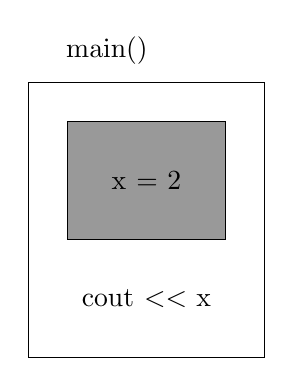
\begin{tikzpicture}
  \def\mywd{3};
  \def\myht{3.5};
  \draw (0,0) rectangle (\mywd,\myht);
  \filldraw[black!40!white,draw=black]%
	(.5,1.5) rectangle (\mywd-.5,\myht-.5)%
	node[black,pos=.5] {\lstinline!x = 2!};
  \node at (1,\myht+.4) {\lstinline!main()!};
  \node at (\mywd/2,.75) {\lstinline!cout << x!};
  \end{tikzpicture}
  \caption{\ref{program:struct:code:scope:example:1} 變數 \lstinline!x! 的可視範圍}
  \label{program:struct:fig:scope:example:1}
\end{subfigure}
~
\begin{subfigure}{.35\textwidth}
  \centering
  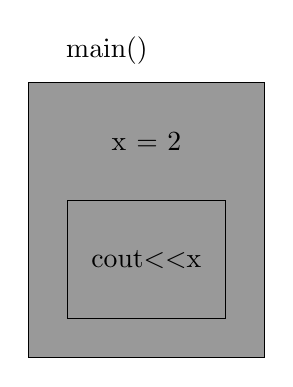
\begin{tikzpicture}
  \def\mywd{3};
  \def\myht{3.5};
  \filldraw[black!40!white,draw=black]%
	(0,0) rectangle (\mywd,\myht);
  \draw (.5,.5) rectangle (\mywd-.5,\myht-1.5)%
	node[pos=.5] {\lstinline!cout<<x!};
  \node at (1,\myht+.4) {\lstinline!main()!};
  \node at (\mywd/2,\myht-.75) {\lstinline!x = 2!};
  \end{tikzpicture}
  \caption{\ref{program:struct:code:scope:example:2} 變數 \lstinline!x! 的可視範圍}
  \label{program:struct:fig:scope:example:2}
\end{subfigure}
\caption{程式碼 \ref{program:struct:code:scope:example} 的狀況}
\label{program:struct:fig:scope:example}
\end{figure}

\paragraph{}變數的可視範圍就像洋蔥一樣,外面一層的變數可以被裡面一層的變數看見,因此程式碼 \ref{program:struct:code:scope:example:1} 的 \lstinline!cout! 沒辦法看見包在大括號的變數 \lstinline!x!。

\paragraph{}程式碼 \ref{program:struct:code:scope:example:2} 展示另外一個例子,結果如圖 \ref{program:struct:fig:scope:example:2},雖然變數 \lstinline!x! 在外層,但裡面的 \lstinline!cout! 會一層一層往外找變數 \lstinline!x!,結果就是輸出 \lstinline!2!。

\subsubsection{選擇結構}

\paragraph{\lstinline!if! 結構}選擇結構在 \texttt{C++} 中就是 \lstinline!if!。\lstinline!if! 最簡單的語法如程式碼 \ref{program:struct:code:if:usage}。

\begin{code}[h!]
\centering
\begin{subcode}{.4\textwidth}
  \centering
  \begin{tabular}{c}
  \begin{lstlisting}
int a = 4;
if (a < 10)
  cout << a << endl;
  \end{lstlisting}
  \end{tabular}
  \caption{單行指令}
  \label{program:struct:code:if:usage:1}
\end{subcode}
~
\begin{subcode}{.4\textwidth}
  \centering
  \begin{tabular}{c}
  \begin{lstlisting}
int a = 4;
if (a < 10) {
  a += 5;
  cout << a << endl;
}
  \end{lstlisting}
  \end{tabular}
  \caption{程式區塊}
  \label{program:struct:code:if:usage:2}
\end{subcode}
\caption{\lstinline!if! 的用法}
\label{program:struct:code:if:usage}
\end{code}

\paragraph{}綜觀兩種情況,在 \lstinline!if! 後面的小括號放\textbf{邏輯運算式},只要邏輯運算式為 \lstinline!true!,就會執行後面的語句,若要執行多行語句,則要使用程式區塊用大括號括好。
\paragraph{}這個結構可以幫助設計一個條件開關,若 \lstinline!true! 執行某些程式;反之,若是 \lstinline!false! 則否。因此程式碼 \ref{program:struct:code:if:usage:1} 第 3 行,和程式碼 \ref{program:struct:code:if:usage:2} 第 3 行至第 5 行會被執行。

\paragraph{\lstinline!if!\texttt{-}\lstinline!else! 結構} 條件判斷可以更進化為 \lstinline!if!\texttt{-}\lstinline!else! 結構,語法如程式碼 \ref{program:struct:code:if:else}。\lstinline!if!\texttt{-}\lstinline!else! 做的是:當邏輯運算式的結果為 \lstinline!true!,執行 \lstinline!if! 的區塊;如果是 \lstinline!false!,則執行 \lstinline!else! 區塊。

\begin{code}[h!]
\centering
\begin{tabular}{c}
\begin{lstlisting}
int a = 4;
if (a < 3)
  cout << "Yes!" << endl;
else
  cout << "QQ" << endl;
\end{lstlisting}
\end{tabular}
\caption{\lstinline!if!\texttt{-}\lstinline!else! 結構}
\label{program:struct:code:if:else}
\end{code}

\paragraph{}同樣地,\lstinline!else! 也可以改為程式區塊。當你要判斷的條件比較多時,\lstinline!if!\texttt{-}\lstinline!else! 可以連用,如程式碼 \ref{program:struct:code:if:else:if}。

\begin{code}[h!]
\centering
\begin{tabular}{c}
\begin{lstlisting}
int a = 4;
if (a < 3)
  cout << "Case 1" << endl;
else if (3 <= a && a < 6)
  cout << "Case 2" << endl;
else
  cout << "Case 3" << endl;
\end{lstlisting}
\end{tabular}
\caption{\lstinline!if! 和 \lstinline!else! 連用}
\label{program:struct:code:if:else:if}
\end{code}

\paragraph{}程式碼 \ref{program:struct:code:if:else:if} 中 \lstinline!if!\texttt{-}\lstinline!else! 可以一直接續下去,除此之外,類似的結構也有 \lstinline!switch! 等,這裡不贅述。


\paragraph{懸置 \lstinline!else! 問題}將程式碼 \ref{program:struct:code:dangling:else:1} 拔掉大括號,變成程式碼 \ref{program:struct:code:dangling:else:2},會有什麼差別?

\begin{code}[h!]
\centering
\begin{subcode}{.5\textwidth}
  \centering
  \begin{tabular}{c}
  \begin{lstlisting}
if (0) {
  if (0) cout << "QQ" << endl;
}
else cout << "XD" << endl;
  \end{lstlisting}
  \end{tabular}
  \caption{危險的 \lstinline!else!}
  \label{program:struct:code:dangling:else:1}
\end{subcode}
~
\begin{subcode}{.45\textwidth}
  \centering
  \begin{tabular}{c}
  \begin{lstlisting}
if (0)
  if (0) cout << "QQ" << endl;
else cout << "XD" << endl;
  \end{lstlisting}
  \end{tabular}
  \caption{編譯器會不知道是哪一個 \lstinline!if! 的 \lstinline!else!}
  \label{program:struct:code:dangling:else:2}
\end{subcode}
\caption{懸置的 \lstinline!else!}
\label{program:struct:code:dangling:else}
\end{code}

\paragraph{}通常沒括大括號的情況下,最後一個 \lstinline!else! 會匹配到最近的 \lstinline!if!,讀者可以驗證這兩段程式碼的不同。

\paragraph{應用:找極值}

\subsubsection{迴圈結構}

\paragraph{比較迴圈結構}

\begin{code}[h!]
\centering
\begin{subcode}{.48\textwidth}
\centering
\begin{tabular}{c}
\begin{lstlisting}
for (int i = 0; i < 10; i++) {
  cout << i << endl;
}
\end{lstlisting}
\end{tabular}
\caption{\lstinline!for! 語法}
\end{subcode}
~
\begin{subcode}{.48\textwidth}
\centering
\begin{tabular}{c}
\begin{lstlisting}
{
  int i = 0;
  while (i < 10) {
    cout << i << endl;
    i++;
  }
}
\end{lstlisting}
\end{tabular}
\caption{對應的 \lstinline!while! 語法}
\end{subcode}
\caption{\lstinline!for! 和 \lstinline!while! 的對應關係}
\label{program:struct:code:loop:for:while}
\end{code}

\paragraph{常見的輸入形式}

\subsubsection{陣列}

\paragraph{}接著來

\subsection{函數}
\subsubsection{傳值呼叫}
\subsubsection{傳址呼叫}
\subsubsection{傳參考呼叫}
\subsubsection{函數多載}
\subsubsection{程式區塊}

\subsection{程式技巧}
\subsubsection{函式化}
\subsubsection{\lstinline!\#define! 與 \lstinline!inline!}

\subsection{\texttt{C++} 物件導向}
\subsubsection{物件與類別}
\subsubsection{建構子與解構子}
\subsubsection{運算子多載}

\subsubsection{命名空間}

\ifx \allfiles \undefined

\printindex

\clearpage
\end{CJK}
\end{document}

\fi